\section{Desarrollo experimental 5}

En este ultimo ejercicio mediremos el factor de potencia en un circuito con control de ángulo de conducción, para ello utilizando el mismo montaje del Experimento 4 ajustamos el ángulo de conducción para que la tensión de salida sea de aproximadamente 110V, luego conectaremos el medidor digital de la siguiente forma:

\begin{figure}[H]
    \centering
    
\includegraphics[width=0.5\textwidth]{images/esquema5.png}
    \caption{Conexiones realizadas}
    \label{fig:conexiones5}
\end{figure}

Obtenemos lo siguiente:

\begin{figure}[H]
    \centering
    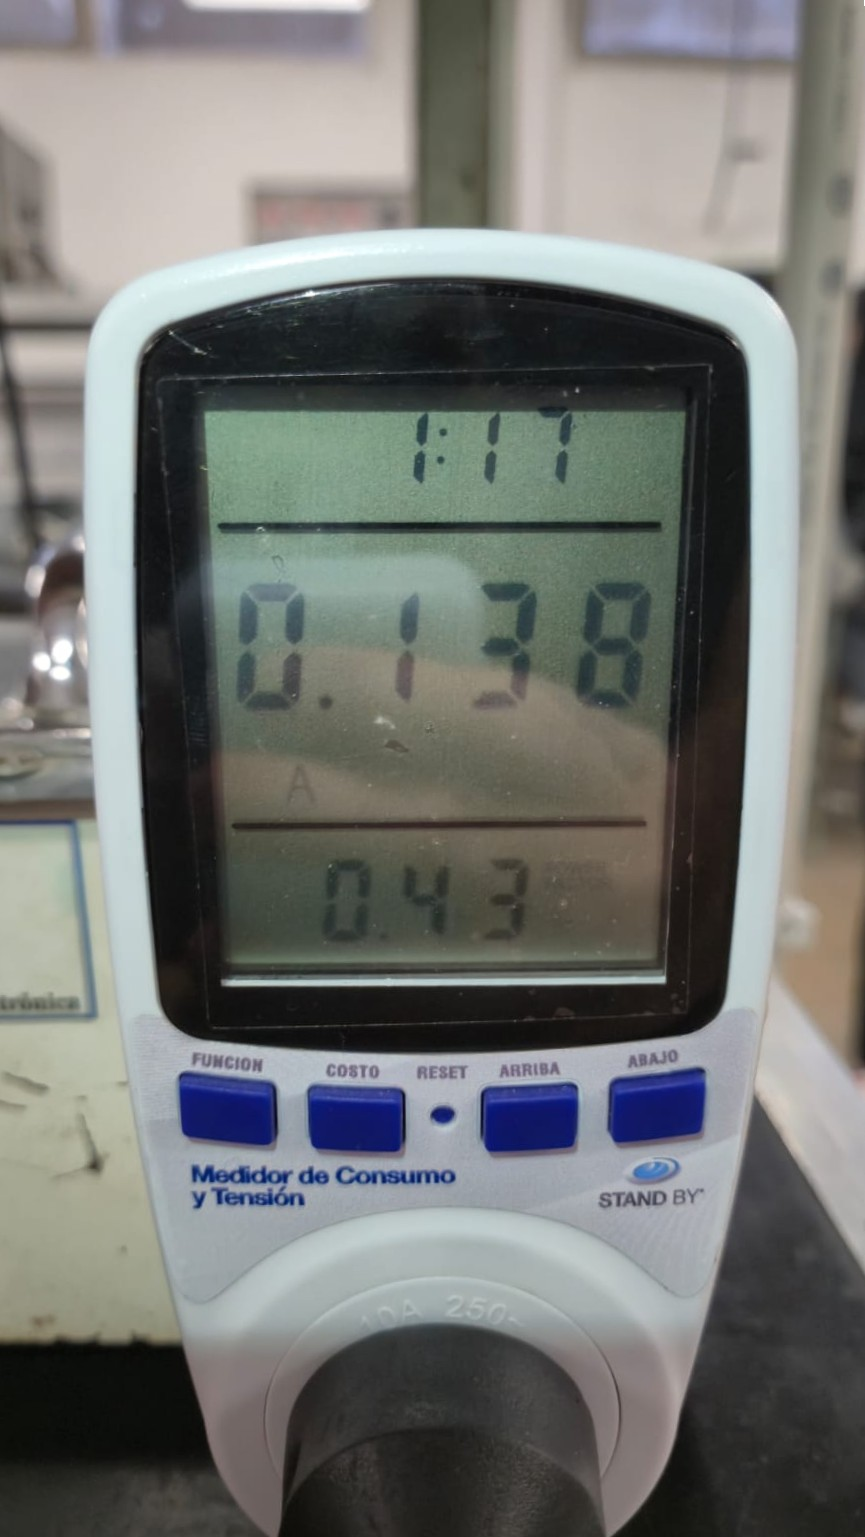
\includegraphics[width=0.5\textwidth]{images/ejercicio5.jpeg}
    \caption{Medición de factor de potencia}
    \label{fig:resistencia5}
\end{figure}